\chapter{Conclusiones}
En este capítulo se presenta el análisis de los resultados obtenidos, las limitaciones encontradas y algunas consideraciones y mejoras para trabajos futuros.

\section{Casos especiales}
Existen algunos casos para los cuales el algoritmo no proporciona un rendimiento adecuado, los cuales se describen a continuación.

\subsection{Iluminación excesiva}
Una iluminación excesiva (\Cref{img:light_1_rgb}) puede crear matices falsos en el canal Hue (\Cref{img:light_1_hue}) lo cual provocará una segmentación incorrecta de la imagen (\Cref{img:light_1_binary}).

\begin{figure}[H]
\centering
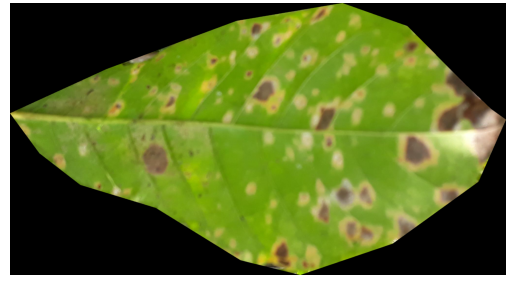
\includegraphics[scale=1]{images/special_case_light_1_rgb.png}
\caption{Iluminación excesiva en una hoja}
\label{img:light_1_rgb}
\end{figure}

\begin{figure}[H]
\centering
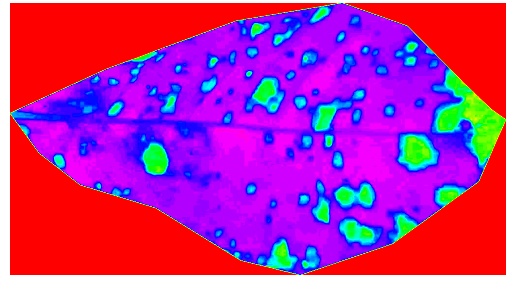
\includegraphics[scale=1]{images/special_case_light_1_hue.png}
\caption{Matices falsos por iluminación excesiva}
\label{img:light_1_hue}
\end{figure}

\begin{figure}[H]
\centering
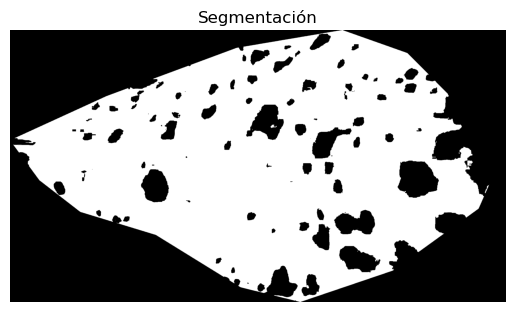
\includegraphics[scale=1]{images/special_case_light_1_binary.png}
\caption{Segmentación de una hoja con iluminación excesiva}
\label{img:light_1_binary}
\end{figure}

\subsection{Iluminación artificial o no contemplada}
De igual manera, una iluminación creada por una fuente artificial (una lámpara) o no contemplada (día nublado), puede causar un despliegue de la imagen inconsistente o contraintuitivo (\Cref{img:light_2_hue}).

\begin{figure}[H]
\centering
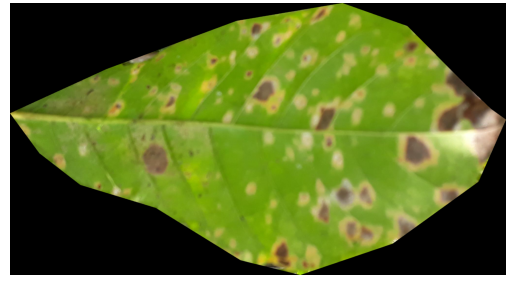
\includegraphics[scale=1]{images/special_case_light_2_rgb.png}
\caption{Hoja con iluminación no contemplada}
\label{img:light_2_rgb}
\end{figure}

\begin{figure}[H]
\centering
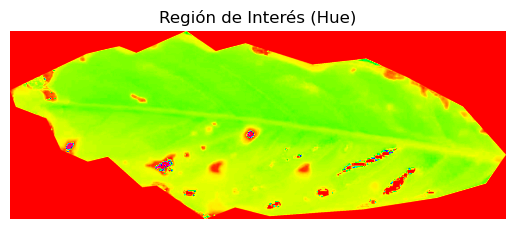
\includegraphics[scale=1]{images/special_case_light_2_hue.png}
\caption{Despliegue contraintuitivo de una imagen}
\label{img:light_2_hue}
\end{figure}

\begin{figure}[H]
\centering
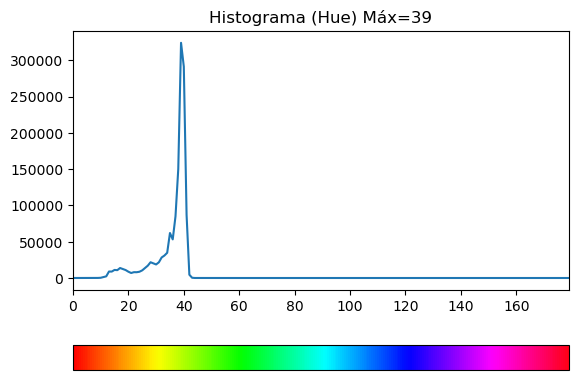
\includegraphics[width=\textwidth]{images/special_case_light_2_histogram.png}
\caption{Histograma de una imagen con despliegue contraintuitivo}
\label{img:light_2_binary}
\end{figure}

\subsection{Envés de la hoja}
El algoritmo ignora el haz y el envés (\Cref{img:backbone_rgb}) de la hoja, por lo tanto, aplica el mismo proceso en ambas condiciones. Sin embargo, los nervios de la hoja presentan, generalmente, un matiz diferente al resto de la hoja (\Cref{img:backbone_hue}), provocando que la segmentación sea errónea (\Cref{img:backbone_binary}).

\begin{figure}[H]
\centering
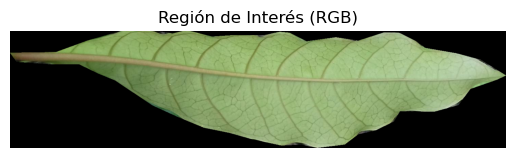
\includegraphics[scale=1]{images/special_case_backbone_rgb.png}
\caption{Envés de una hoja saludable}
\label{img:backbone_rgb}
\end{figure}

\begin{figure}[H]
\centering
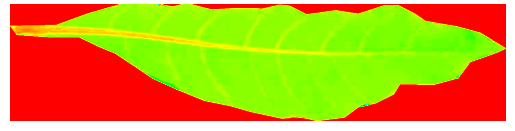
\includegraphics[scale=1]{images/special_case_backbone_hue.png}
\caption{Canal Hue del envés de una hoja saludable}
\label{img:backbone_hue}
\end{figure}

\begin{figure}[H]
\centering

\includegraphics[scale=1]{images/special_case_backbone_binary.png}
\caption{Segmentación del envés de una hoja saludable}
\label{img:backbone_binary}
\end{figure}

\section{Mejoras y trabajo a futuro}

\begin{enumerate}

\item Detección de objetos.

Actualmente el algoritmo se apoya en las anotaciones del dataset para la determinación del contorno de las hojas y la creación de la máscara. Sin embargo, el aislamiento no es preciso e introduce ruido al sistema.

La \Cref{img:issue_countour_rgb} muestra el contorno asignado a una hoja saludable el cual no es preciso e introduce matices no deseados en el canal Hue (\Cref{img:issue_countour_hue}) provocando una segmentación incorrecta de la imagen (\Cref{img:issue_countour_binary}).

\begin{figure}[H]
\centering
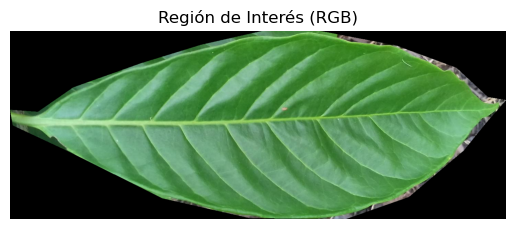
\includegraphics[scale=1]{images/consideration_contour_rgb.png}
\caption{Contorno impreciso de una hoja saludable}
\label{img:issue_countour_rgb}
\end{figure}

\begin{figure}[H]
\centering
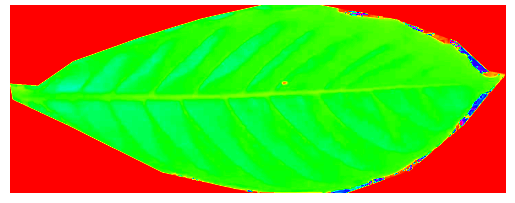
\includegraphics[scale=1]{images/consideration_contour_hue.png}
\caption{Matices no deseados en un contorno impreciso}
\label{img:issue_countour_hue}
\end{figure}

\begin{figure}[H]
\centering

\includegraphics[scale=1]{images/consideration_contour_binary.png}
\caption{Introducción de zonas afectadas debido a un contorno impreciso}
\label{img:issue_countour_binary}
\end{figure}

Una mejora sugerida para resolver este problema es la creación de un algoritmo (o método) para la detección de objetos que permita aislar la región de interés de manera precisa mejorando el rendimiento global del algoritmo.

\item Optimización de los umbrales de segmentación.

Los umbrales de segmentación sugeridos en la \Cref{table:recommended_segmentation} fueron calculados manualmente a través de un enfoque de prueba y error. Por lo tanto, pueden existir umbrales que mejoran el rendimiento del algoritmo.

Una forma automatizada de encontrar umbrales más eficientes, o de verificar que no los hay, es mediante el uso de algoritmos genéticos. Este proceso identificaría la configuración más eficiente de los umbrales maximizando su nivel de eficiencia, o bien, reduciendo el margen de error.

\item Análisis en \textsf{RGB}.

A pesar de que la segmentación por matices en el canal Hue es útil para la detección de zonas afectadas, no nos proporciona información acerca de la severidad en la zona, o si bien lo hace, tal información es fácil de confundirse con otras propiedades que generan matices similares (\Cref{img:issue_severity_hue}).

Existen casos en que una hoja presenta un área mínima de afectación pero con una severidad muy alta (\Cref{img:issue_severity_rgb}) catalogándola automáticamente como severamente afectada. En otras palabras, el área afectada (\Cref{img:issue_severity_binary}) no es suficiente para la clasificación correcta de la hoja.

Una segmentación basada en colores \textsf{RGB} podría ser más eficaz e intuitiva para estos casos.

\begin{figure}[H]
\centering
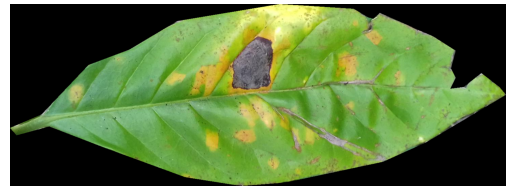
\includegraphics[scale=1]{images/consideration_severity_rgb.png}
\caption{Hoja de café con afectación severa en zona reducida}
\label{img:issue_severity_rgb}
\end{figure}

\begin{figure}[H]
\centering
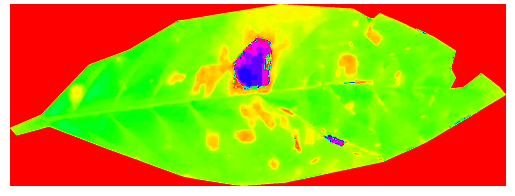
\includegraphics[scale=1]{images/consideration_severity_hue.png}
\caption{Canal Hue de afectación severa en zona reducida}
\label{img:issue_severity_hue}
\end{figure}

\begin{figure}[H]
\centering
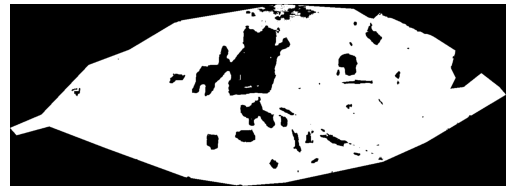
\includegraphics[scale=1]{images/consideration_severity_binary.png}
\caption{Área afectada de una hoja con afectación severa en zona reducida}
\label{img:issue_severity_binary}
\end{figure}

\end{enumerate}

\section{Conclusiones específicas}

\begin{enumerate}
\item No existe una solución única.

El algoritmo no provee una solución general, es decir, dependiendo de la clasificación de las hojas que se desea buscar o analizar, debería elegirse umbrales de segmentación diferentes. La \Cref{table:recommended_segmentation} proporciona la mejor configuración encontrada para cada una de las categorías establecidas.

\begin{table}[H]
\centering
\begin{tabular}{|l|c|c|}
\hline 
\textbf{Clasificación} & \textbf{Umbral de segmentación} & \textbf{Eficiencia \%}\\ 
\hline 
healthy & 25 - 120 & 71.175 \\ 
\hline 
rust\_level\_1 & 30 - 100 & 58.72 \\ 
\hline 
rust\_level\_2 & 30 - 80 & 44.578 \\ 
\hline 
rust\_level\_3 & 40 - 80 & 35.483 \\ 
\hline 
rust\_level\_4 & 40 - 80/120 & 40.00 \\ 
\hline 
\end{tabular}
\caption{Umbrales de segmentación recomendados}
\label{table:recommended_segmentation}
\end{table}

\item El dataset presenta inconsistencias.

Parte de la ineficiencia del algoritmo se debe a que algunas anotaciones en el dataset fueron mal etiquetadas:

\begin{figure}[H]
\centering
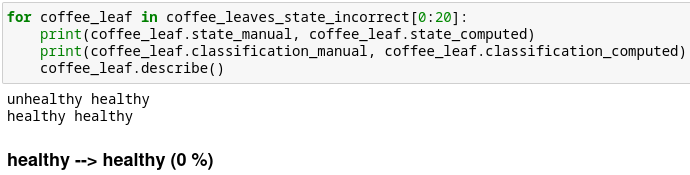
\includegraphics[width=\textwidth]{images/consideration_tag_error.png}
\caption{Inconsistencias en el dataset}
\label{img:dataset_inconsistencies}
\end{figure}

No puede suceder que la clasificación de una hoja sea marcada como saludable mientras que su estado sea no-saludable (\Cref{img:dataset_inconsistencies}). Se encontraron \textbf{4} inconsistencias en el dataset (descartando la categoría \textit{araña roja}).

\end{enumerate}

\section{Conclusiones generales}
Un procesamiento digital de imágenes tradicional generalmente es más eficiente cuando el campo u objeto de estudio es reducido y está normalizado, es decir, no hay mucha variabilidad en las condiciones que describen al sistema.

Este tipo de procesamiento nos da la flexibilidad de poder controlar las características a analizar o identificar de manera precisa, sin embargo, es eso mismo lo que lo hace menos portable o escalable ya que para nuevas condiciones en el sistema, el algoritmo deberá ser ajustado, implicando un alto grado de supervisión humana.

Cabe mencionar que podemos mejorar estos algoritmos tanto como sea necesario para hacerlos más precisos y aumentar su eficiencia pero hay que considerar el tiempo de desarrollo y el costo computacional agregado.